% questions.tex —— 2017 年·天津卷·理科 · 题目内容片段（无答案）
% 由 tools/generate_projects.py 依来源总账自 2017/2017_数学真题_天津理_试题.md 生成，勿手改（改源 MD 后重跑）

\gkpart{数学}

\begin{gktip}
\textbf{来源说明}：本题面依据固定源 PDF 两页 A3 页面逐题核对，原卷印刷页码 1055–1056。固定源不附答案；本文件仅为题面规范源。
\end{gktip}

\gkpart{一、选择题}

\begin{question}
\gkti{1}
设集合 $A=\{1,2,4,6\}$，$B=\{2,4\}$，$C=\{x\in\mathbb R\mid -1\leqslant x\leqslant5\}$，则 $(A\cup B)\cap C=$（　）

\begin{itemize}
\item (A) $\{2\}$
\item (B) $\{1,2,4\}$
\item (C) $\{1,2,4,5\}$
\item (D) $\{x\in\mathbb R\mid -1\leqslant x\leqslant5\}$
\end{itemize}

\end{question}
\begin{question}
\gkti{2}
\Needspace{5\baselineskip}
设变量 $x,y$ 满足约束条件
\nopagebreak[4]
\[
\begin{cases}
2x+y\geqslant0,\\
x+2y-2\geqslant0,\\
x\leqslant0,\\
y\leqslant3,
\end{cases}
\]
则目标函数 $z=x+y$ 的最大值为（　）

\begin{itemize}
\item (A) $\dfrac23$
\item (B) $1$
\item (C) $\dfrac32$
\item (D) $3$
\end{itemize}

\Needspace{0.4\textheight}
\end{question}
\begingroup
\renewenvironment{question}{\Needspace{0.5\textheight}}{}
\begin{question}
\gkti{3}

阅读程序框图，运行相应的程序，若输入 $N$ 的值为 $24$，则输出 $N$ 的值为（　）
\nopagebreak[4]
\begin{center}\begin{tikzpicture}[>=stealth,thick,
  term/.style={draw,rounded corners=3pt,minimum width=21mm,minimum height=7mm},
  proc/.style={draw,minimum width=28mm,minimum height=8mm,align=center},
  test/.style={draw,diamond,aspect=2.35,inner sep=1pt,align=center},
  io/.style={draw,trapezium,trapezium left angle=70,trapezium right angle=110,
    minimum width=25mm,minimum height=8mm,align=center}]
  \node[term] (start) at (0,0) {开始};
  \node[io] (input) at (0,-1.15) {输入 $N$};
  \node[test] (div) at (0,-2.65) {$N$ 能被 $3$ 整除？};
  \node[proc] (divide) at (-2.9,-4.5) {$N=N/3$};
  \node[proc] (minus) at (2.9,-4.5) {$N=N-1$};
  \node[test] (small) at (0,-5.55) {$N\leq 3$？};
  \node[io] (output) at (0,-7.05) {输出 $N$};
  \node[term] (stop) at (0,-8.2) {结束};
  \draw[->] (start)--(input);
  \draw[->] (input)--(div);
  \draw[->] (div.south)--(0,-3.8)--(-2.9,-3.8)--(divide.north);
  \node at (.38,-3.55) {是};
  \draw[->] (div.east)--node[above]{否} ++(1.0,0)|-(minus.north);
  \draw[->] (divide.south)|-(small.west);
  \draw[->] (minus.south)|-(small.east);
  \draw[->] (small.south)--node[right]{是}(output.north);
  \draw[->] (output)--(stop);
  \draw[->] (small.west)--(-3.8,-5.55)--node[pos=.78,left]{否}(-3.8,-2.65)--(div.west);
\end{tikzpicture}
\end{center}
\nopagebreak[4]
\begin{itemize}
\item (A) $0$
\item (B) $1$
\item (C) $2$
\item (D) $3$
\end{itemize}

\end{question}
\endgroup
\begin{question}
\gkti{4}
设 $\theta\in\mathbb R$，则“$\left|\theta-\dfrac\pi{12}\right|<\dfrac\pi{12}$”是“$\sin\theta<\dfrac12$”的（　）

\begin{itemize}
\item (A) 充分而不必要条件
\item (B) 必要而不充分条件
\item (C) 充要条件
\item (D) 既不充分也不必要条件
\end{itemize}

\end{question}
\begin{question}
\gkti{5}
已知双曲线 $\dfrac{x^2}{a^2}-\dfrac{y^2}{b^2}=1\ (a>0,b>0)$ 的左焦点为 $F$，离心率为 $\sqrt2$。若经过 $F$ 和 $P(0,4)$ 两点的直线平行于双曲线的一条渐近线，则双曲线的方程为（　）

\begin{itemize}
\item (A) $\dfrac{x^2}{4}-\dfrac{y^2}{4}=1$
\item (B) $\dfrac{x^2}{8}-\dfrac{y^2}{8}=1$
\item (C) $\dfrac{x^2}{4}-\dfrac{y^2}{8}=1$
\item (D) $\dfrac{x^2}{8}-\dfrac{y^2}{4}=1$
\end{itemize}

\end{question}
\begin{question}
\gkti{6}
已知奇函数 $f(x)$ 在 $\mathbb R$ 上是增函数，$g(x)=xf(x)$。若 $a=g(-\log_2 5.1)$，$b=g(2^{0.8})$，$c=g(3)$，则 $a,b,c$ 的大小关系为（　）

\begin{itemize}
\item (A) $a<b<c$
\item (B) $c<b<a$
\item (C) $b<a<c$
\item (D) $b<c<a$
\end{itemize}

\end{question}
\begin{question}
\gkti{7}
设函数 $f(x)=2\sin(\omega x+\varphi)$，$x\in\mathbb R$，其中 $\omega>0$，$|\varphi|<\pi$。若 $f\left(\dfrac{5\pi}{8}\right)=2$，$f\left(\dfrac{11\pi}{8}\right)=0$，且 $f(x)$ 的最小正周期大于 $2\pi$，则（　）

\begin{itemize}
\item (A) $\omega=\dfrac23,\ \varphi=\dfrac\pi{12}$
\item (B) $\omega=\dfrac23,\ \varphi=-\dfrac{11\pi}{12}$
\item (C) $\omega=\dfrac13,\ \varphi=-\dfrac{11\pi}{24}$
\item (D) $\omega=\dfrac13,\ \varphi=\dfrac{7\pi}{24}$
\end{itemize}

\end{question}
\begin{question}
\gkti{8}
\Needspace{5\baselineskip}
已知函数
\nopagebreak[4]
\[
f(x)=
\begin{cases}
x^2-x+3,&x\leqslant1,\\
x+\dfrac2x,&x>1,
\end{cases}
\]
设 $a\in\mathbb R$，若关于 $x$ 的不等式 $f(x)\geqslant\left|\dfrac x2+a\right|$ 在 $\mathbb R$ 上恒成立，则 $a$ 的取值范围是（　）

\begin{itemize}
\item (A) $\left[-\dfrac{47}{16},2\right]$
\item (B) $\left[-\dfrac{47}{16},\dfrac{39}{16}\right]$
\item (C) $[-2\sqrt3,2]$
\item (D) $\left[-2\sqrt3,\dfrac{39}{16}\right]$
\end{itemize}

\end{question}
\gkpart{二、填空题}

\begin{question}
\gkti{9}
已知 $a\in\mathbb R$，$i$ 为虚数单位，若 $\dfrac{a-i}{2+i}$ 为实数，则 $a$ 的值为\gkblank{}。

\end{question}
\begin{question}
\gkti{10}
已知一个正方体的所有顶点在一个球面上，若这个正方体的表面积为 $18$，则这个球的体积为\gkblank{}。

\end{question}
\begin{question}
\gkti{11}
在极坐标系中，直线 $4\rho\cos\left(\theta-\dfrac\pi6\right)+1=0$ 与圆 $\rho=2\sin\theta$ 的公共点的个数为\gkblank{}。

\end{question}
\begin{question}
\gkti{12}
若 $a,b\in\mathbb R$，$ab>0$，则 $\dfrac{a^4+4b^4+1}{ab}$ 的最小值为\gkblank{}。

\end{question}
\begin{question}
\gkti{13}
在 $\triangle ABC$ 中，$\angle A=60^\circ$，$AB=3$，$AC=2$。若 $\overrightarrow{BD}=2\overrightarrow{DC}$，$\overrightarrow{AE}=\lambda\overrightarrow{AC}-\overrightarrow{AB}\ (\lambda\in\mathbb R)$，且 $\overrightarrow{AD}\cdot\overrightarrow{AE}=-4$，则 $\lambda$ 的值为\gkblank{}。

\end{question}
\begin{question}
\gkti{14}
用数字 $1,2,3,4,5,6,7,8,9$ 组成没有重复数字，且至多有一个数字是偶数的四位数，这样的四位数一共有\gkblank{}个。（用数字作答）

\end{question}
\gkpart{三、解答题}

\begin{question}
\gkti{15}
在 $\triangle ABC$ 中，内角 $A,B,C$ 所对的边分别为 $a,b,c$。已知 $a>b$，$a=5$，$c=6$，$\sin B=\dfrac35$。

(1)   求 $b$ 和 $\sin A$ 的值；
(2)   求 $\sin\left(2A+\dfrac\pi4\right)$ 的值。

\end{question}
\begin{question}
\gkti{16}
从甲地到乙地要经过 3 个丁字路口，设各路口信号灯工作相互独立，且在各路口遇到红灯的概率分别为 $\dfrac12,\dfrac13,\dfrac14$。

(1)   设 $X$ 表示一辆车从甲地到乙地遇到红灯的个数，求随机变量 $X$ 的分布列和数学期望；
(2)   若有 2 辆车独立地从甲地到乙地，求这 2 辆车共遇到 1 个红灯的概率。

\Needspace{0.4\textheight}
\end{question}
\begin{question}
\gkti{17}
如图，在三棱锥 $P-ABC$ 中，$PA\perp$ 底面 $ABC$，$\angle BAC=90^\circ$。点 $D,E,N$ 分别为棱 $PA,PC,BC$ 的中点，$M$ 是线段 $AD$ 的中点，$PA=AC=4$，$AB=2$。
\nopagebreak[4]
\begin{center}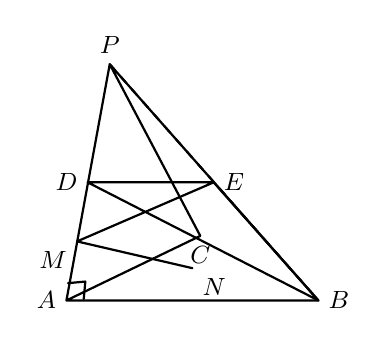
\begin{tikzpicture}[thick,line cap=round,line join=round,
  every node/.style={font=\small}]
  \coordinate (P) at (0,3.0);
  \coordinate (A) at (-.55,0);
  \coordinate (B) at (2.65,0);
  \coordinate (C) at (1.15,.82);
  \coordinate (D) at (-.28,1.5);
  \coordinate (E) at (1.32,1.5);
  \coordinate (N) at (1.05,.41);
  \coordinate (M) at (-.415,.75);
  % Outer pyramid and source-visible internal segments. The right-angle mark
  % is at A, as printed; no unlabelled construction point is added.
  \draw (P)--(A)--(B)--(P) (A)--(C) (P)--(C);
  \draw (B)--(D) (D)--(E) (B)--(E) (E)--(M) (M)--(N);
  \draw[dashed] (P)--(B);
  \draw (A) ++(.22,.02)--++(.02,.22)--++(-.22,-.02);
  \node[above] at (P) {$P$};
  \node[left] at (A) {$A$};
  \node[right] at (B) {$B$};
  \node[below] at (C) {$C$};
  \node[left] at (D) {$D$};
  \node[right] at (E) {$E$};
  \node[below left] at (M) {$M$};
  \node[below right] at (N) {$N$};
\end{tikzpicture}
\end{center}
\nopagebreak[4]
(1)   求证：$MN\parallel$ 平面 $BDE$；
(2)   求二面角 $C-EM-N$ 的正弦值；
(3)   已知点 $H$ 在棱 $PA$ 上，且直线 $NH$ 与直线 $BE$ 所成角的余弦值为 $\dfrac{\sqrt7}{21}$，求线段 $AH$ 的长。

\end{question}
\begin{question}
\gkti{18}
已知 $\{a_n\}$ 为等差数列，前 $n$ 项和为 $S_n\ (n\in\mathbb N^*)$，$\{b_n\}$ 是首项为 $2$ 的等比数列，且公比大于 $0$，$b_2+b_3=12$，$b_3=a_4-2a_1$，$S_{11}=11b_4$。

(1)   求 $\{a_n\}$ 和 $\{b_n\}$ 的通项公式；
(2)   求数列 $\{a_{2n}b_{2n-1}\}$ 的前 $n$ 项和 $\ (n\in\mathbb N^*)$。

\end{question}
\begin{question}
\gkti{19}
设椭圆 $\dfrac{x^2}{a^2}+\dfrac{y^2}{b^2}=1\ (a>b>0)$ 的左焦点为 $F$，右顶点为 $A$，离心率为 $\dfrac12$。已知 $A$ 是抛物线 $y^2=2px\ (p>0)$ 的焦点，$F$ 到抛物线的准线 $l$ 的距离为 $\dfrac12$。

(1)   求椭圆的方程和抛物线的方程；
(2)   设 $l$ 上两点 $P,Q$ 关于 $x$ 轴对称，直线 $AP$ 与椭圆相交于点 $B\ (B$ 异于 $A)$，直线 $BQ$ 与 $x$ 轴相交于点 $D$。若 $\triangle APD$ 的面积为 $\dfrac{\sqrt6}{2}$，求直线 $AP$ 的方程。

\end{question}
\begin{question}
\gkti{20}
\Needspace{5\baselineskip}
设 $a\in\mathbb Z$，已知定义在 $\mathbb R$ 上的函数
\nopagebreak[4]
\[
f(x)=2x^4+3x^3-3x^2-6x+a
\]
在区间 $(1,2)$ 内有一个零点 $x_0$，$g(x)$ 为 $f(x)$ 的导函数。

(1)   求 $g(x)$ 的单调区间；
(2)   设 $m\in[1,x_0)\cup(x_0,2]$，函数 $h(x)=g(x)(m-x_0)-f(m)$，求证：$h(m)h(x_0)<0$；
\Needspace{5\baselineskip}
(3)   求证：存在大于 $0$ 的常数 $A$，使得对于任意的正整数 $p,q$，且 $\dfrac pq\in[1,x_0)\cup(x_0,2]$，满足
\nopagebreak[4]
\[
\left|\frac pq-x_0\right|\geqslant\frac1{Aq^4}.
\]

\end{question}